\begin{figure}

\centering

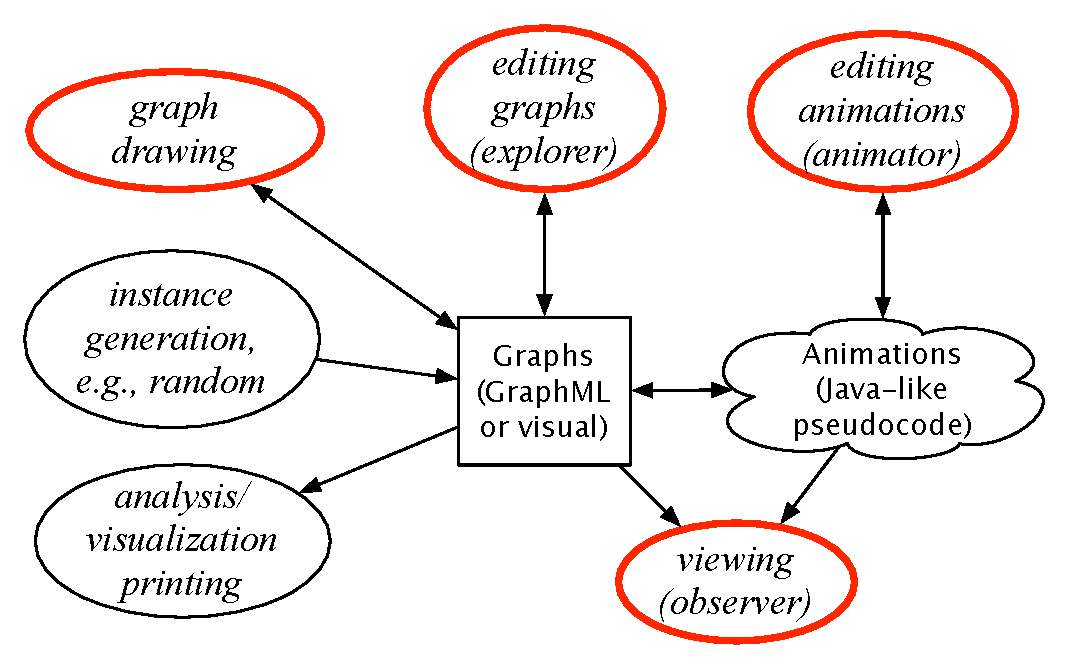
\includegraphics[width=\columnwidth]{X_overview_diagram}

\caption{Illustration of Galant design and functionality. Arrows indicate
  data flow. All functions, shown as ovals can be performed easily outside of
Galant. The ones with thick red borders are part of current Galant
functionality.}

\label{fig:overview_diagram}
\end{figure}

% [Last modified: 2013 06 25 at 16:04:45 GMT]


Fig.~\ref{fig:overview_diagram} gives an overview of Galant functionality.
A graphical user interface (GUI) allows the user to edit both graphs and
algorithm animations, either loaded as already existing files or newly
created. At any point, the user can apply a selected animation to a selected
graph for viewing.
The animation program 
steps forward until it
displays the next animation event or, if a \texttt{beginStep()}
call has marked the start of a sequence of events, until
it reaches the next \texttt{endStep()} call.
It then pauses execution and waits for the user to decide whether to
step forward, step backward, or exit.
A step forward resumes execution while a step backward returns the display to a previous
state.
The algorithm resumes execution only when the \emph{display state}
indicated by the user's sequence of forward and backward steps
($f-b$, where $f$ is the number of forward and $b$ the number of backward steps)
exceeds the \emph{algorithm state}, the number of animation steps the algorithm
has executed.

When editing a graph the user can create/delete nodes and edges (when in the appropriate mode)
by clicking and/or
moving the mouse, and can move vertices by dragging the mouse.
There is also an interface for specifying labels, weights and colors for both
nodes and edges.
Keyboard shortcuts are available for these operations.
 
A preferences panel allows the user to select font size for labels and a
variety of other options.
Any changes to a graph are also reflected in a text (GraphML) representation
of the graph, which can also be edited directly. Naturally the GraphML
representation can also be created or edited externally: by a random or
structured graph generator, by translation from another format, by directly
editing the GraphML or by invoking a separate graph editor.
Galant has a built-in force-directed drawing program 
(the one reported by Hu~\cite{2006-Mathematica-Hu}) to position nodes
automatically if so desired.
Automatic drawing is useful when the input Graphml file does not provide position
information for the nodes (and their positions are selected randomly).
Other drawing programs, such as those provided by GraphViz~\cite{GraphViz}
and the huge body of research carried on by the graph drawing community~\cite{graph_drawing},
can be used externally as well.
Graphs used in Galant animations
can be analyzed externally using tools such as Gephi~\cite{gephi}.

Editing/compiling an algorithm animation is just like performing the same
operations on a Java program.
The compiler is essentially a Java
compiler that preprocesses the algorithm code
and compiles it, importing the relevant modules.
The preprocessor converts traversals of incidence lists and other
lists of nodes or edges into the corresponding, more obscure, Java code.
It also shields the Galant programmer from such syntactic circumlocutions
as declaring \texttt{static} methods.
Because the functionality of the Galant editor is limited, it is usually more
convenient to use an external program editor, reserving the Galant editor to
make minor changes in response to compile-time or runtime errors.

We use GraphML~\cite{GraphML} as our graph representation because it is flexible, it can
easily be extended, and parsers, viewers and translation tools are becoming
more common.
Because GraphML is
specialized XML, parsers for the latter, based on the Document Object Model
(DOM) can be used. These are available for many programming languages.
Translators to other formats are also available or can easily be constructed.
For example, the GraphViz~\cite{GraphViz} download provides one;
unfortunately it preserves
only
the connectivity information.
However, there is straightforward mapping between the GraphML attributes we
use (positions of nodes and colors, etc., of nodes and edges) and the
corresponding ones in GraphViz format.
Translators to and from other formats are also available or can easily be constructed.
We have written conversion scripts among the following formats:
GraphML, gml~\cite{1999-TRPassau-Himsolt}, sgf, and dot (GraphViz~\cite{GraphViz}).
The sgf (simple graph) format was devised by the first author as a
lingua franca specific to layered graphs.
It is similar to the \texttt{gr} format used in the 9th DIMACS implementation
challenge~\cite{2006-DIMACS-Implementation}
except that layer and position are used instead of x- and y-coordinates
and
there are no weights on the edges.
When layered graphs are represented using
dot files these are supplemented with \emph{ord} files
that give layer and position information for nodes
-- see Stallmann et al.~\cite{2001-JEA-Stallmann}.

% [Last modified: 2013 06 25 at 18:06:12 GMT]
